%fiber2chip_modelings
As beginning of this chapter the waveguide model will be approximate with a rectangle waveguide. Place the waveguide at the working distance $4\mu$m before the TLF.  Fig.\quad\ref{fig:coupling_e_field} from the simulation of this configuration shows the E-Field spread more widely at the interface of the waveguide than that in the case without blockage of the waveguide and apparently a great part of E-Field infiltrate into the waveguide rather than accepted by guide. Thus by checking the S-parameter of this simulation Fig.\ref{fig:orignial_coupling_efficiency},which present the S21 in frequencies, the coupling efficiency ($S_{21}$) is about $48.8\%$ at the working frequency $282$HZ($\lambda=1064$nm). This result will act as the reference sample for the other simulations. 
\begin{figure}[!ht]
\centering
	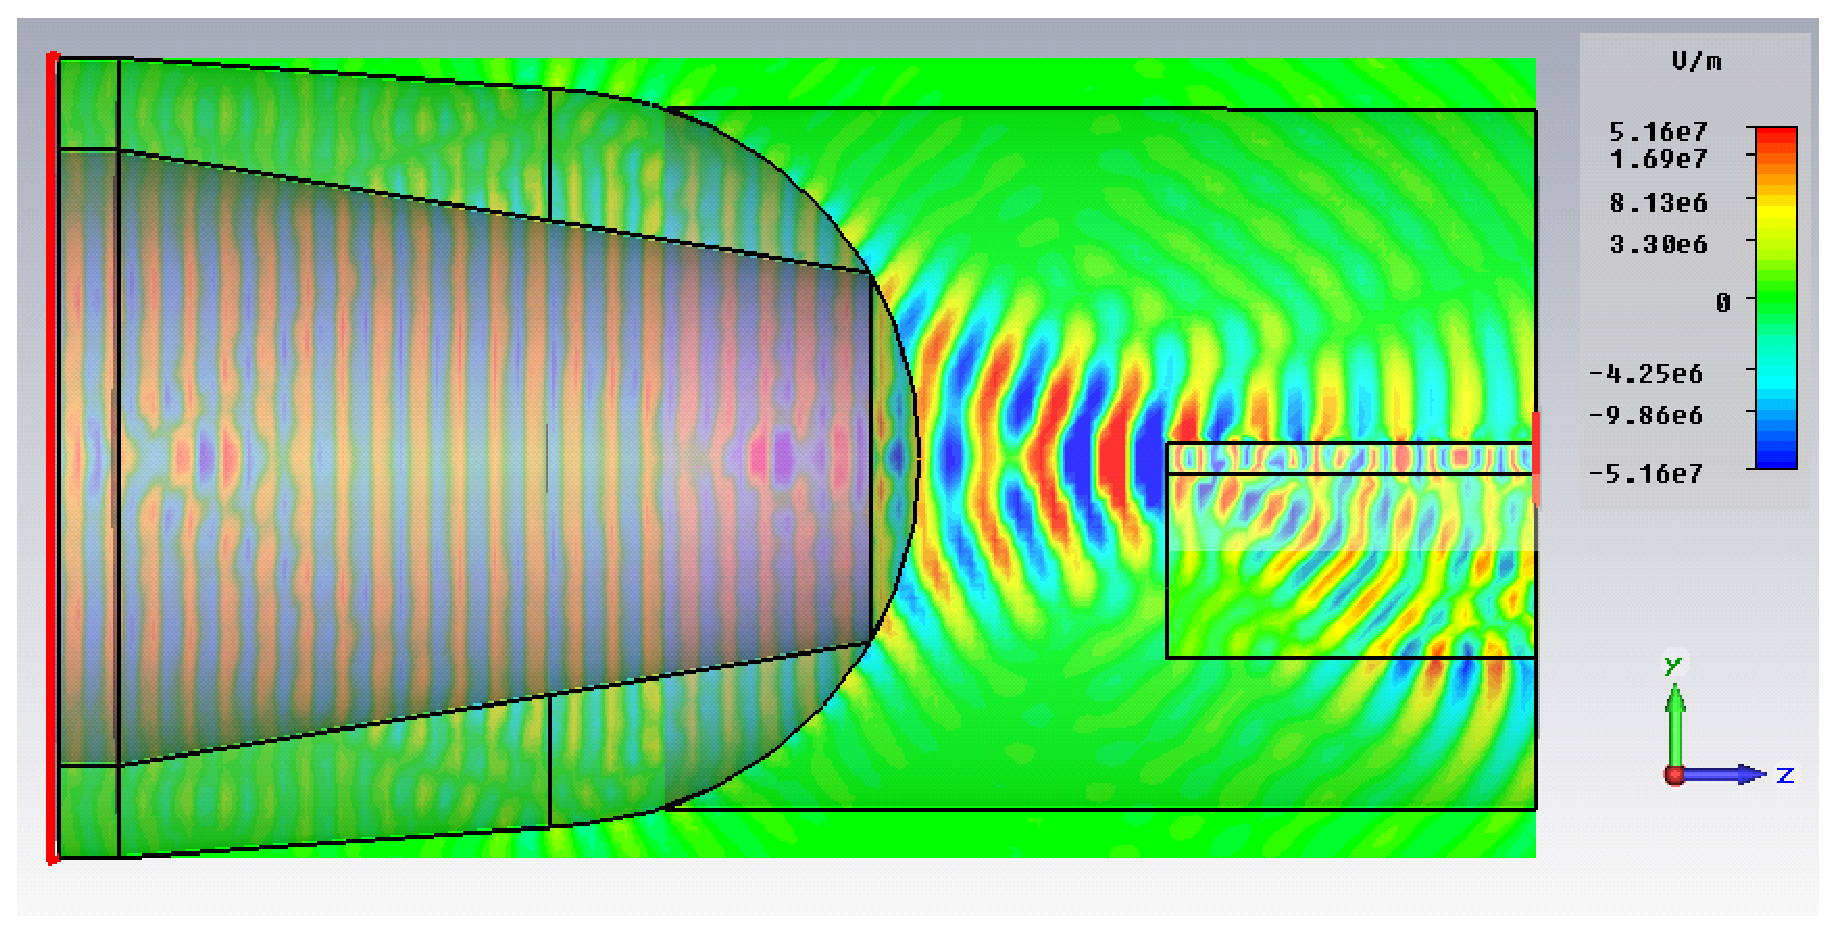
\includegraphics[width=0.7 \textwidth]{bilder/cst_basic_waveguide_efield}
	\label{fig:coupling_e_field}
	\caption{E-Field demonstration by coupling.}
\end{figure}
Furthermore people can analyze the power distribution at the guide from Fig.\quad\ref{fig:power_distribution}( see Appendix.\quad\ref{app:powwer_distribution} ). In the figure it can be found that about $40\%$ power propagates in the guide while another $40\%$ in the substrate and the rest is losing in the air or reflecting.
\begin{figure}
\centering
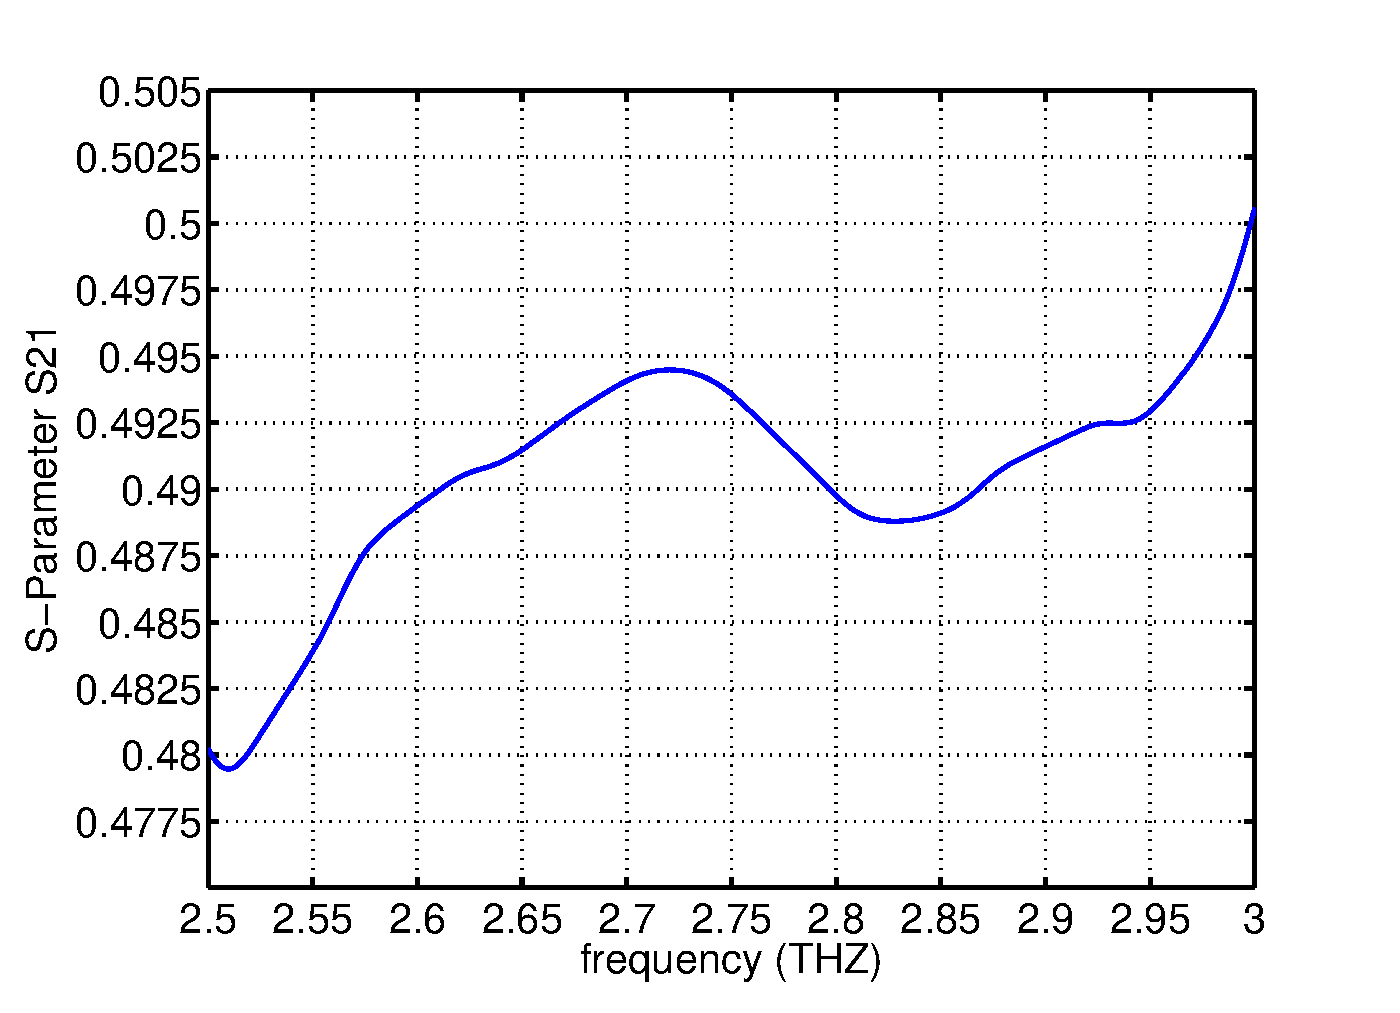
\includegraphics[width=0.7\textwidth]{bilder/original_coupling_efficiency}
\caption{coupling efficiency in Frequency area.}
\label{fig:orignial_coupling_efficiency}
\end{figure}
\begin{figure}[!ht]
\centering
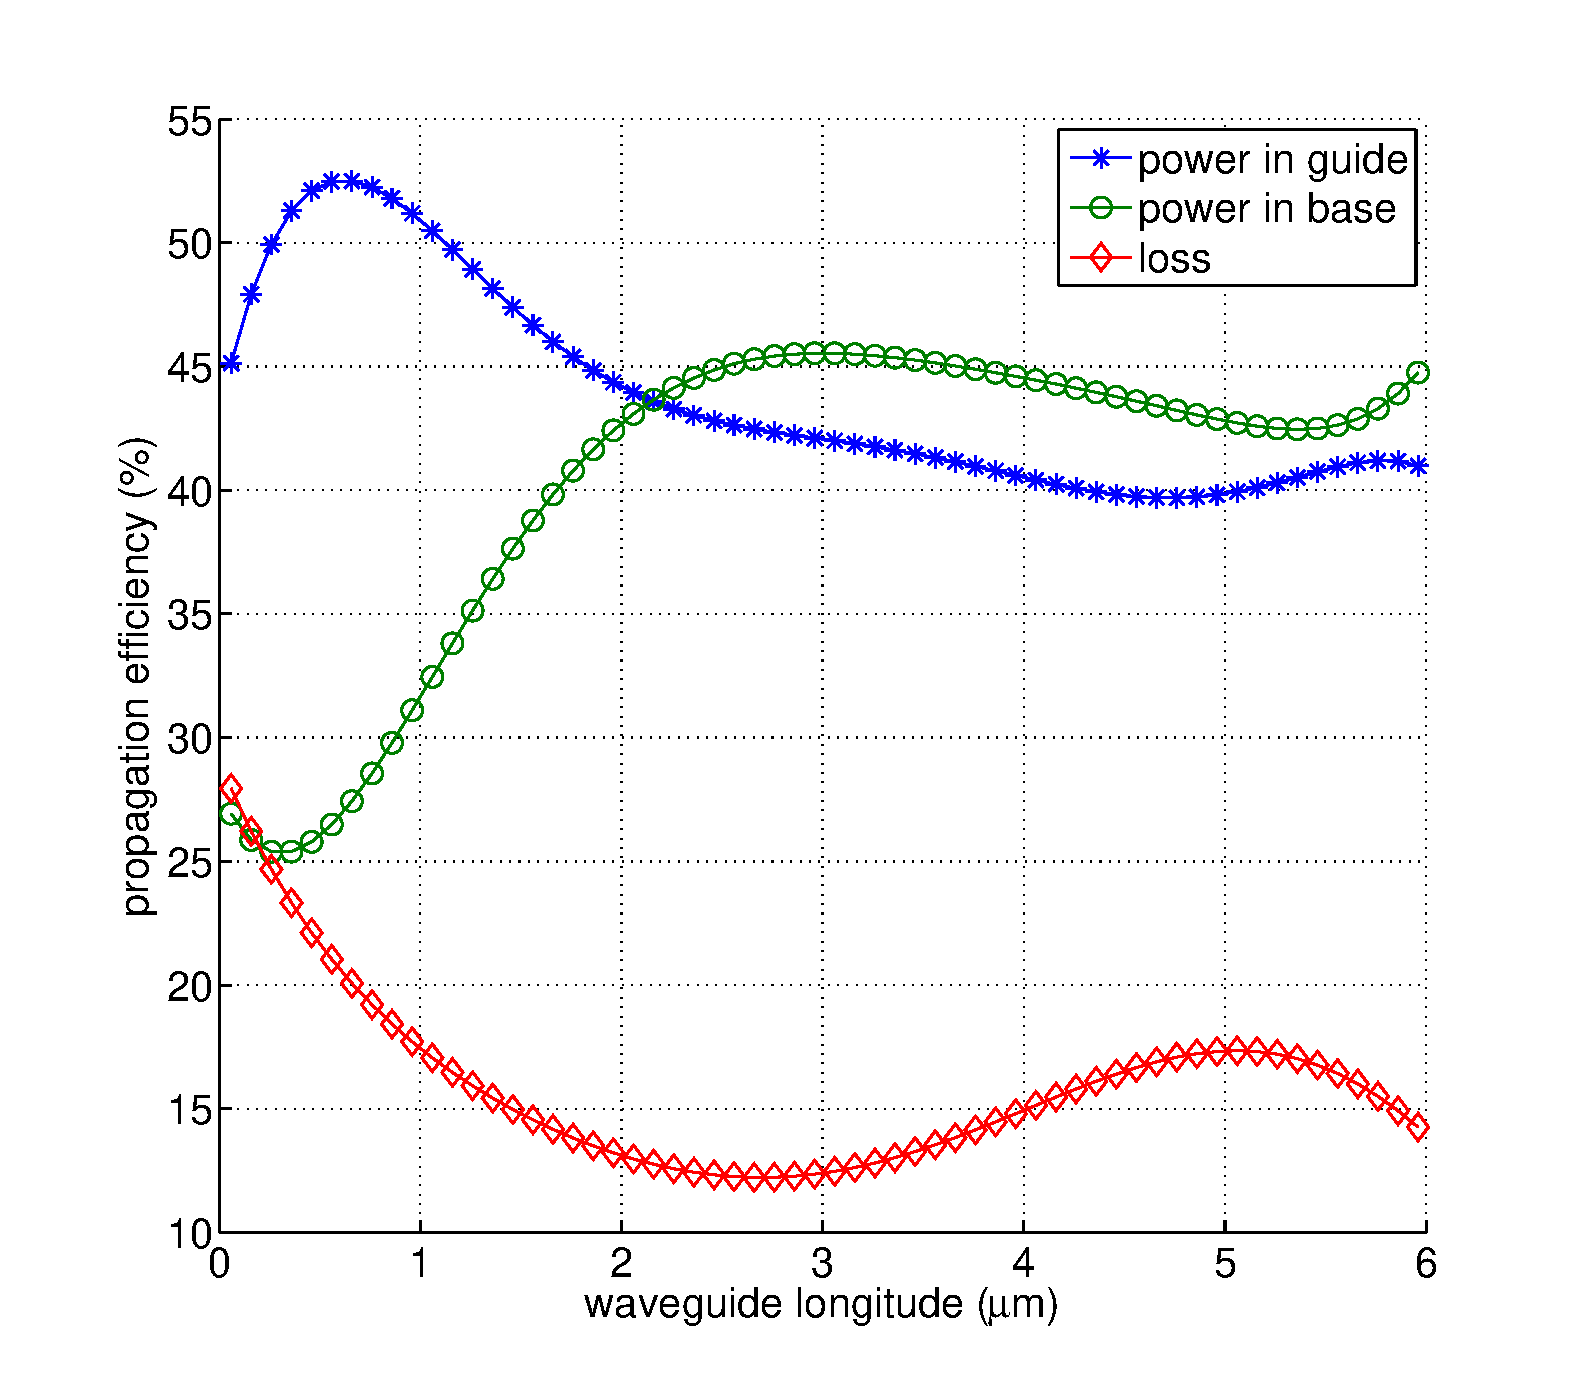
\includegraphics[width=0.7\textwidth]{bilder/power_distribution1}
\caption{power distribution along the waveguide.}
\label{fig:power_distribution}
\end{figure}
